% ------------------------------------------------------------------------------
% TYPO3 CMS 7.3 - What's New - Chapter "Introduction" (English Version)
%
% @author	Michael Schams <schams.net>
% @license	Creative Commons BY-NC-SA 3.0
% @link		http://typo3.org/download/release-notes/whats-new/
% @language	English
% ------------------------------------------------------------------------------
% LTXE-CHAPTER-UID:		066dde91-8cd613b5-0eadb76c-a6245b74
% LTXE-CHAPTER-NAME:	Introduction
% ------------------------------------------------------------------------------

\section{Введение}
\begin{frame}[fragile]
	\frametitle{Введение}

	\begin{center}\huge{Введение}\end{center}
	\begin{center}\huge{\color{typo3darkgrey}\textbf{Факты}}\end{center}

\end{frame}

% ------------------------------------------------------------------------------
% LTXE-SLIDE-START
% LTXE-SLIDE-UID:		baf14aa0-791f1c0c-3e525632-3269ce52
% LTXE-SLIDE-ORIGIN:	1c3389b6-2103f93f-b2319a3e-aacc6eba English
% LTXE-SLIDE-ORIGIN:	6d5e9f3e-f9d9677e-43d7d497-e80ba9ef German
% LTXE-SLIDE-TITLE:		TYPO3 CMS 7.3 - The Facts
% ------------------------------------------------------------------------------
\begin{frame}[fragile]
	\frametitle{Введение}
	\framesubtitle{TYPO3 CMS 7.3 - факты}

	\begin{itemize}
		\item Дата выхода: 16 июня 2015
		\item Тип: "Sprint Release"
		\item Направленность: охват, инновации, доступность
		\item Фокус: экосистема пакетов, Composer и обработка расширений
	\end{itemize}

\end{frame}

% ------------------------------------------------------------------------------
% LTXE-SLIDE-START
% LTXE-SLIDE-UID:		9e634370-95f89439-d5d3a4fb-a969edad
% LTXE-SLIDE-ORIGIN:	780b1e6f-e761ec98-824890a3-8d429b56 English
% LTXE-SLIDE-ORIGIN:	759c3860-d5061f6e-2bb0009f-6ea130c8 German
% LTXE-SLIDE-TITLE:		System Requirements
% ------------------------------------------------------------------------------
\begin{frame}[fragile]
	\frametitle{Введение}
	\framesubtitle{Системные требования}

	\begin{itemize}
		\item PHP*:\tabto{4cm}v5.5.0 - v5.6.x
		\item MySQL:\tabto{4cm}v5.5.x - v5.6.x (no strict mode)
		\item Дисковое пространство:\tabto{4cm}мин. 200 МБ
		\item PHP настройки:

			\begin{itemize}
				\item memory\_limit >= 128M
				\item max\_execution\_time >= 240s
				\item параметр компиляции \texttt{--disable-ipv6} \underline{не} должен использоваться
			\end{itemize}

		\item Внутренний интерфейс требует IE >= 9 или любой другой современный браузер

	\end{itemize}

	\vspace{1cm}
	*) Подробности: \href{http://typo3.org/news/article/php-minimum-requirements-for-typo3-cms-7/}{PHP Minimum Requirements for TYPO3 CMS 7}

\end{frame}

% ------------------------------------------------------------------------------
% LTXE-SLIDE-START
% LTXE-SLIDE-UID:		20763dbb-78a6cdae-83557d71-a75a1400
% LTXE-SLIDE-ORIGIN:	e06c97c6-ee283664-40fe3fe5-af3a1caa English
% LTXE-SLIDE-ORIGIN:	70c77c41-e2b83d82-2f182996-98061070 German
% LTXE-SLIDE-TITLE:		Development And Release Timeline
% ------------------------------------------------------------------------------
\begin{frame}[fragile]
	\frametitle{Введение}
	\framesubtitle{График разработки и выхода}

	\begin{figure}
		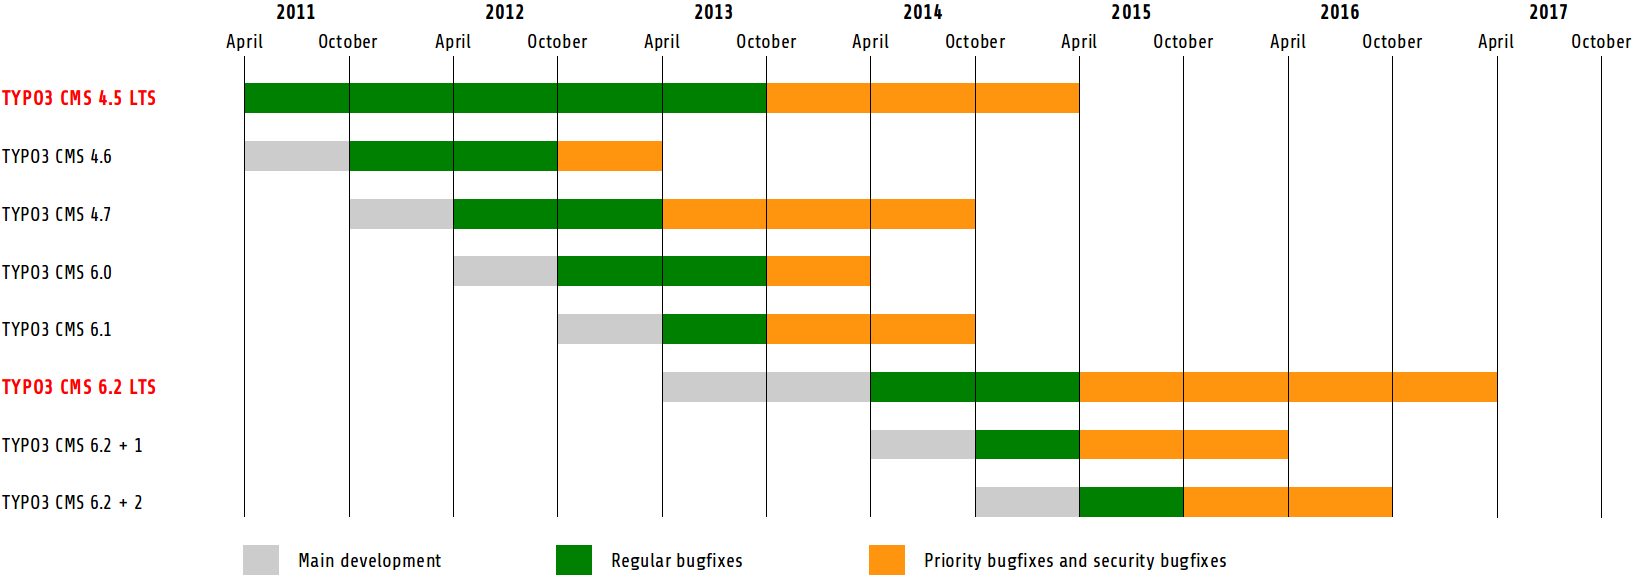
\includegraphics[width=0.90\linewidth]{Introduction/ReleaseAgenda.png}
	\end{figure}

\end{frame}

% ------------------------------------------------------------------------------
% LTXE-SLIDE-START
% LTXE-SLIDE-UID:		55924a41-af0af3b2-36c28eb6-547ff3e8
% LTXE-SLIDE-ORIGIN:	cfdf68b1-b00a3fca-0adf0630-7563d7da English
% LTXE-SLIDE-ORIGIN:	b55d3fe9-76807061-d97f3fee-7db1f190 German
% LTXE-SLIDE-TITLE:		TYPO3 CMS Roadmap
% ------------------------------------------------------------------------------
\begin{frame}[fragile]
	\frametitle{Введение}
	\framesubtitle{Маршрутная карта TYPO3 CMS}

	Примерные даты выхода и их направленность:

	\begin{itemize}
		\item v7.0 \tabto{1.0cm}02/Dec/2014\tabto{3.4cm}Переработка внутреннего интерфейса часть 1
		\item v7.1 \tabto{1.0cm}24/Feb/2015\tabto{3.4cm}Чистка ядра и оптимизация
		\item v7.2 \tabto{1.0cm}28/Apr/2015\tabto{3.4cm}Внешний интерфейс

		\item
			\begingroup
				\color{typo3orange}
					v7.3 \tabto{1.0cm}16/Jun/2015\tabto{3.4cm}Экосистема пакетов, Composer\newline
                    \tabto{3.4cm}и работа с расширениями
			\endgroup

		\item v7.4 \tabto{1.0cm}04/Aug/2015\tabto{3.4cm}Переработка внутреннего интерфейса часть 2
		\item v7.5 \tabto{1.0cm}29/Sep/2015\tabto{3.4cm}\textit{(будет определено...)}
		\item v7.6 \tabto{1.0cm}xx/xxx/2015\tabto{3.4cm}\textbf{TYPO3 CMS 7 LTS} (Long Term Release)
	\end{itemize}

	\smaller
		\url{https://typo3.org/typo3-cms/roadmap/}\newline
		\url{http://typo3.org/news/article/embrace-and-innovate-typo3-cms-7/}
	\normalsize

\end{frame}

% ------------------------------------------------------------------------------
% LTXE-SLIDE-START
% LTXE-SLIDE-UID:		e0fcac53-45053e8f-bfcb3bfa-16551e47
% LTXE-SLIDE-ORIGIN:	eb02037c-0fba04b6-5006d3f3-03fe223a English
% LTXE-SLIDE-ORIGIN:	b0c28f26-c3ca2e99-195954a8-ed76f9d4 German
% LTXE-SLIDE-TITLE:		Installation
% ------------------------------------------------------------------------------
\begin{frame}[fragile]
	\frametitle{Введение}
	\framesubtitle{Установка}

	\begin{itemize}
		\item Официальная процедура установки под Linux/Mac OS X\newline
			(DocumentRoot, например \texttt{/var/www/site/htdocs}):
		\begin{lstlisting}
			$ cd /var/www/site
			$ wget --content-disposition get.typo3.org/7.3
			$ tar xzf typo3_src-7.3.0.tar.gz
			$ cd htdocs
			$ ln -s ../typo3_src-7.3.0 typo3_src
			$ ln -s typo3_src/index.php
			$ ln -s typo3_src/typo3
			$ touch FIRST_INSTALL
		\end{lstlisting}

		\item Symbolic links под Microsoft Windows:

			\begin{itemize}
				\item Используйте \texttt{junction} под Windows XP/2000
				\item Используйте \texttt{mlink} под Windows Vista и Windows 7
			\end{itemize}

	\end{itemize}
\end{frame}

% ------------------------------------------------------------------------------
% LTXE-SLIDE-START
% LTXE-SLIDE-UID:		edeeae93-4df1d553-c7c17f84-bf7eb4ff
% LTXE-SLIDE-ORIGIN:	5c2e0134-2f1f18d2-55b74162-25dd3995 English
% LTXE-SLIDE-ORIGIN:	48136734-ae508d23-bce5811d-667f8908 German
% LTXE-SLIDE-TITLE:		Upgrade to TYPO3 CMS 7
% ------------------------------------------------------------------------------
\begin{frame}[fragile]
	\frametitle{Введение}
	\framesubtitle{Обновление до TYPO3 CMS 7.x}

	\begin{itemize}
		\item Обновление возможно лишь с TYPO3 CMS 6.2 LTS
		\item Сначала TYPO3 CMS < 6.2 необходимо обновить до TYPO3 CMS 6.2 LTS
	\end{itemize}

	\begin{itemize}

		\item Инструкции по обновлению:\newline
			\smaller\url{http://wiki.typo3.org/Upgrade#Upgrading_to_7.3}\normalsize
		\item Официальное руководство TYPO3 "TYPO3 Installation and Upgrading":
			\smaller\url{http://docs.typo3.org/typo3cms/InstallationGuide}\normalsize
		\item Общий подход:
			\begin{itemize}
				\item \smaller Проверка минимальных системных требований \small(PHP, MySQL и т. д.)
				\item \smaller Просмотр \textbf{deprecation\_*.log} из старой установки TYPO3
				\item \smaller Обновление всех расширений до последних версий
				\item \smaller Загрузка новых исходных файлов и запуск Install Tool \textrightarrow Upgrade Wizard
				\item \smaller Обзор модулей, запускаемых для внутренних пользователей (не обязательно)
			\end{itemize}
	\end{itemize}

\end{frame}

% ------------------------------------------------------------------------------
